\section{Results}\label{sec:results}
We first report the main case against the original comparators (Section~\ref{sec:main}). We then report the decisive test, against rules re-calibrated on a large budget (Section~\ref{sec:robust}), and what happens at seed level (Section~\ref{sec:seeds}). Further checks follow (Section~\ref{sec:checks}), then the settings where the learner did not help (Section~\ref{sec:nohelp}) and what the policy actually does (Section~\ref{sec:behaviour}). Table~\ref{tab:summary} in Section~\ref{sec:discussion} collects the main numbers.

\subsection{Main case: deadline traffic with delayed HARQ feedback (M1)}\label{sec:main}
The residual A2C policy delivers \NMonePctPrim\,\% of packets on time in M1, against \NMonePctCtx\,\% for the Context table, \NMonePctFixed\,\% for Fixed and \NMonePctOLLA\,\% for OLLA (Fig.~\ref{fig:thesis}, Table~\ref{tab:m1}). Its margin is \NMonePrimOLLAMar\,\% over OLLA, \NMonePrimFixedMar\,\% over Fixed and \NMonePrimCtxMar\,\% over the Context table (\NLevTrace\,\% CI [\NMonePrimCtxLo, \NMonePrimCtxHi]\,\%), the strongest of the original rules. In absolute terms the last margin is \NMoneAbsPpCtx{} percentage points. The policy beats all nine comparators under the trace-level rule, and it does so without hurting fairness: the Jain index changes by \NMoneJainDiff{} and the 5th-percentile user improves by \NMoneEdgePct\,\% against the Context table.

How much of the gain over OLLA do simple calibrated rules already capture? A single calibrated offset (Fixed) captures \NMoneCalibShareFixed\,\% of the learner's gain over OLLA, and the Context table \NMoneCalibShareCtx\,\%. A comparison against OLLA alone would therefore overstate what the learner adds. These original rules were calibrated on only \NCfgCalib{} or \NCfgCalibCtx{} traces; the next subsection replaces them with rules calibrated on \NGsixCalTraces{} traces.

\begin{figure}[t]
\centering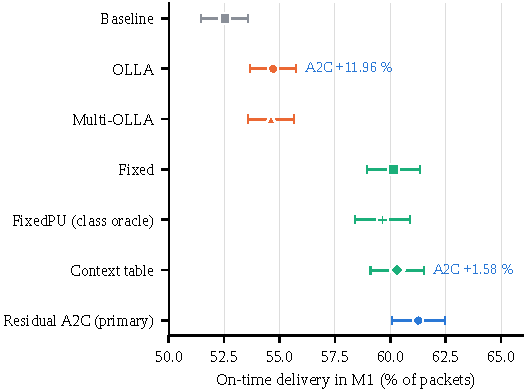
\includegraphics[width=\columnwidth]{f1_thesis}
\caption{M1 on-time delivery ratio by scheme (mean and \NLevHier\,\% CI over \NCfgEval{} traces). Blue: residual A2C; orange: OLLA family; green: calibrated rules; gray: baseline. Annotations give the margin of the learned policy.}\label{fig:thesis}
\end{figure}

\begin{table*}[t]
\caption{M1 against the original comparators. Margin: paired percentage gain of residual A2C over the comparator, with the \NLevTrace\,\% CI over traces and the Holm-adjusted Wilcoxon $p$. ``Beats'': the trace-level rule is met. The tuned-target OLLA selected the default target in M1, and the two bandits coincide. Re-calibrated comparators are in Table~\ref{tab:g6}.}\label{tab:m1}
\centering\footnotesize
\begin{tabular}{@{}lcccrc@{}}
\toprule
Comparator & On-time (\%) & Margin (\%) & \NLevTrace\,\% CI (\%) & Holm $p$ & Beats\\
\midrule
Baseline & \NMonePctBaseline & \NMonePrimBaselineMar & [\NMonePrimBaselineLo, \NMonePrimBaselineHi] & \NMonePrimBaselineHolm & \NMonePrimBaselineBeats\\
OLLA & \NMonePctOLLA & \NMonePrimOLLAMar & [\NMonePrimOLLALo, \NMonePrimOLLAHi] & \NMonePrimOLLAHolm & \NMonePrimOLLABeats\\
OLLA (tuned target) & \NMonePctOLLAT & \NMonePrimOLLATMar & [\NMonePrimOLLATLo, \NMonePrimOLLATHi] & \NMonePrimOLLATHolm & \NMonePrimOLLATBeats\\
Multi-OLLA & \NMonePctMulti & \NMonePrimMultiMar & [\NMonePrimMultiLo, \NMonePrimMultiHi] & \NMonePrimMultiHolm & \NMonePrimMultiBeats\\
Bandit (global) & \NMonePctBanG & \NMonePrimBanGMar & [\NMonePrimBanGLo, \NMonePrimBanGHi] & \NMonePrimBanGHolm & \NMonePrimBanGBeats\\
Bandit (delay class) & \NMonePctBanD & \NMonePrimBanDMar & [\NMonePrimBanDLo, \NMonePrimBanDHi] & \NMonePrimBanDHolm & \NMonePrimBanDBeats\\
Fixed & \NMonePctFixed & \NMonePrimFixedMar & [\NMonePrimFixedLo, \NMonePrimFixedHi] & \NMonePrimFixedHolm & \NMonePrimFixedBeats\\
FixedPU (class oracle) & \NMonePctFPU & \NMonePrimFPUMar & [\NMonePrimFPULo, \NMonePrimFPUHi] & \NMonePrimFPUHolm & \NMonePrimFPUBeats\\
Context table & \NMonePctCtx & \NMonePrimCtxMar & [\NMonePrimCtxLo, \NMonePrimCtxHi] & \NMonePrimCtxHolm & \NMonePrimCtxBeats\\
\bottomrule
\end{tabular}
\end{table*}

\begin{figure*}[t]
\centering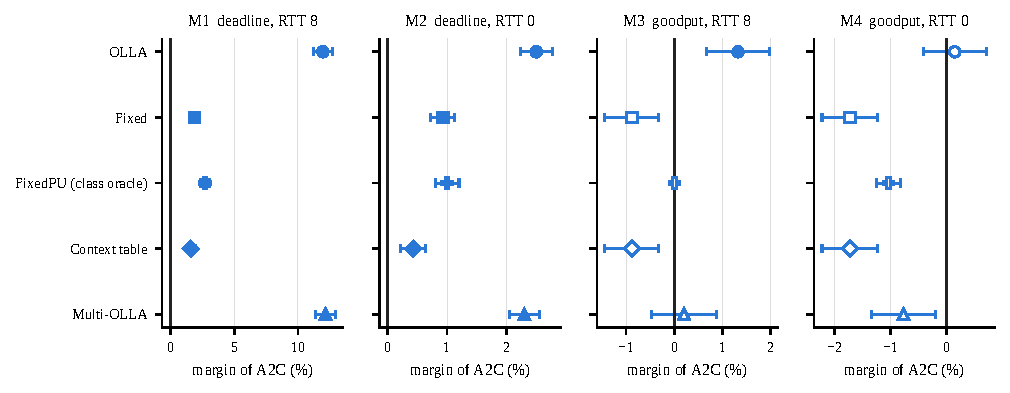
\includegraphics[width=\textwidth]{f3_forest}
\caption{Margin of residual A2C over each original comparator in the four cases (\NLevTrace\,\% CI over traces). Filled markers: the trace-level rule is met; open markers: it is not. The two bandits are omitted for scale (see Table~\ref{tab:m1}).}\label{fig:forest}
\end{figure*}

\subsection{The decisive test: re-calibrated comparators}\label{sec:robust}
The original rules had a small calibration budget, and two of their searches were incomplete (Section~\ref{sec:protocol}). The re-calibration study gives every rule \NGsixCalTraces{} fresh calibration traces, disjoint from the evaluation traces, and searches Fixed, the Context table and the tuned-target OLLA exhaustively. It also adds a stronger rule, the \emph{combined table}: one CQI offset for each combination of deadline slack, delay class, speed class and busy HARQ processes (\NGsixCells{} cells, Appendix~\ref{app:g6}). The combined table uses the same cues as the learner and its base rule, including the oracle speed class. All tables were frozen and hashed before any evaluation trace was run. They also show no sign of over-fitting: the combined table scores \NGsixCalCtxJ{} on the calibration traces and \NGsixEvalCtxJ{} on the evaluation traces.

Table~\ref{tab:g6} and Fig.~\ref{fig:robust}a give the result. The learned policy still beats every re-calibrated rule on the evaluation traces: by \NGsixCtxDMar\,\% over the re-calibrated Context table and \NGsixFixedDMar\,\% over the re-calibrated Fixed offset. \emph{Over the combined table, however, the margin is only \NGsixCtxJMar\,\%} (\NLevTrace\,\% CI [\NGsixCtxJLo, \NGsixCtxJHi]\,\%), or \NGsixAbsPpCtxJ{} percentage points. Compared with the \NMonePrimCtxMar\,\% over the original Context table, re-calibration and the combined table remove \NGsixClosure\,\% of the learner's margin over the best rule. Most of what looked like a learning advantage is available to a deterministic table calibrated carefully on the same cues.

Two remarks qualify the combined table. It was expensive to find: the coordinate-ascent search took \NGsixSearchHours~h of simulation, against \NMoneHours~h to train and evaluate the ten learned policies. And one of its \NGsixStarts{} search starts stopped at the safety cap while still improving (Appendix~\ref{app:g6}). If anything the table is slightly under-optimised, which favours the learner.

\begin{table*}[t]
\caption{The learned policy (M1) against comparators re-calibrated on \NGsixCalTraces{} fresh traces, on the \NCfgEval{} M1 evaluation traces. Trace level: margin, \NLevTrace\,\% CI and Holm-adjusted $p$ over these \NGsixNcmp{} comparators. Seed level: seeds with a positive margin, hierarchical seed$\times$trace \NLevHier\,\% CI, and whether the seed-level rule is met (lower bound above zero).}\label{tab:g6}
\centering\footnotesize
\begin{tabular}{@{}lccccccc@{}}
\toprule
& \multicolumn{4}{c}{Trace level} & \multicolumn{3}{c}{Seed level}\\
\cmidrule(lr){2-5}\cmidrule(l){6-8}
Comparator & Margin (\%) & \NLevTrace\,\% CI (\%) & Holm $p$ & Beats & Seeds $>\lit{0}$ & Hier.\ \NLevHier\,\% CI (\%) & Robust\\
\midrule
\inputtab{gen/tab_g6.tex}
\bottomrule
\end{tabular}
\end{table*}

\subsection{Seed-level robustness}\label{sec:seeds}
Trace-level intervals treat the ten trained policies as fixed. A practitioner, however, trains one policy, so we also ask how the margin varies across training seeds (Fig.~\ref{fig:seeds}).

\emph{Against the original rules the result is robust.} Against the original Context table \NGMoneCtxAbove{} of \NMoneSeedsTotal{} seeds are above zero (one-sided sign test $p=\NGMoneCtxSign$), and the hierarchical seed$\times$trace \NLevHier\,\% interval is [\NGMoneCtxHierLo, \NGMoneCtxHierHi]\,\%. Against Fixed it is [\NGMoneFixedHierLo, \NGMoneFixedHierHi]\,\%. The same holds against every re-calibrated single-cue rule (Table~\ref{tab:g6}).

\emph{Against the combined table it is not.} Only \NGsixCtxJAbove{} of \NCfgSeeds{} seeds beat the combined table (sign test $p=\NGsixCtxJSign$), and the hierarchical interval is [\NGsixCtxJHierLo, \NGsixCtxJHierHi]\,\%. Under the pre-registered seed-level rule the margin is therefore \emph{not robust to seed resampling}. The probability that a randomly chosen trained policy beats the table on a randomly chosen trace~\cite{agarwal2021precipice} is \NGsixCtxJPoI{} (\NLevHier\,\% CI [\NGsixCtxJPoILo, \NGsixCtxJPoIHi]), close to a coin flip. The trace-level result also fails a Bonferroni correction over all tests in the project ($p=\NBonfPCtxJ$, Section~\ref{sec:protocol}). The automatic summary of the re-calibration stage had marked the result as seed-robust, because it applied the seed-level rule to the re-calibrated Context table only; the rule requires the strongest comparator, and we report the corrected verdict.

The hierarchical intervals are about \NGWidthRatio{} times wider than trace-only ones, which is the price of counting seed variance. A deterministic ensemble of the ten seeds (a secondary scheme) reaches \NGsixValEns{} on time, which shows how much of the spread an ensemble removes; it was not part of the pre-registered decision.

\begin{figure}[t]
\centering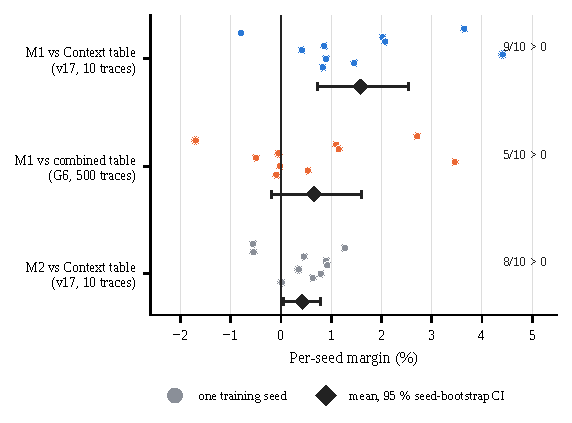
\includegraphics[width=\columnwidth]{f4_seeds}
\caption{Per-seed margins (one dot per training seed) with the mean and its \NLevHier\,\% bootstrap interval over seed means (diamond). Top: M1 against the original Context table. Middle: M1 against the combined table. Bottom: M2 against the original Context table. The count of seeds above zero is given on the right.}\label{fig:seeds}
\end{figure}

\subsection{Further checks}\label{sec:checks}
\begin{figure*}[t]
\centering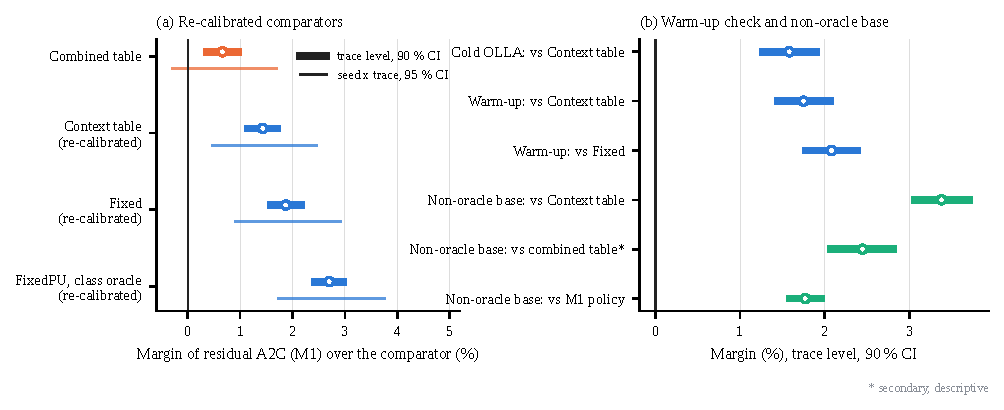
\includegraphics[width=\textwidth]{f6_robust}
\caption{(a) Margin of the learned policy over the re-calibrated comparators; thick bars: trace-level \NLevTrace\,\% CI; thin bars: hierarchical seed$\times$trace \NLevHier\,\% CI. Orange: the seed-level interval includes zero. (b) Warm-up check (OLLA warmed up for \NWoneTTI{} TTIs) and non-oracle base ablation; trace-level \NLevTrace\,\% CIs. The ablation has no seed-level interval because per-seed values were not stored.}\label{fig:robust}
\end{figure*}

\subsubsection{Does OLLA just need time to converge?}
OLLA starts each trace cold, and only \NCfgScored{} TTIs are scored. In the warm-up check all loops run for \NWoneTTI{} TTIs before scoring. The margin over OLLA falls from \NWoneOLLAColdMar\,\% to \NWoneOLLAWarmMar\,\% (\NLevTrace\,\% CI [\NWoneOLLAWarmLo, \NWoneOLLAWarmHi]\,\%), so part of the gap to OLLA was its convergence time. The learner itself barely changes (\NWoneValCold{} cold, \NWoneValWarm{} warm). Against the calibrated rules the warm-up changes little: \NWoneCtxWarmMar\,\% over the Context table and \NWoneFixedWarmMar\,\% over Fixed. As pre-registered, the abstract quotes the smaller, warm-up gain over OLLA.

\subsubsection{A non-oracle configuration (NR1, NR2)}
The M1 policy acts on FixedPU, whose offsets use the true speed class. The non-oracle base ablation (NR1) retrains the same recipe on the Fixed base (one global offset of \NNRoneOff{} CQI steps, the same value as the re-calibrated Fixed rule), with fresh training seeds. The learner's own state is gNB-observable, so this configuration uses no oracle information at all. It delivers \NNRoneVal{} on time, beats all \NNRoneWins{} original comparators (\NNRoneCtxMar\,\% over the Context table) and is \NNRoneMoneMar\,\% above the M1 policy ([\NNRoneMoneLo, \NNRoneMoneHi]\,\%; Fig.~\ref{fig:robust}b). \wordingsel{NR1}{NR}{verdict}{unrun} A secondary comparison on the same traces puts it \NNRoneGCtxJMar\,\% above the combined table ([\NNRoneGCtxJLo, \NNRoneGCtxJHi]\,\%).

Because NR1 reused M1's evaluation traces and did not store per-seed values, a pre-registered confirmatory replication (NR2) was conducted with \lit{500} fresh evaluation traces, \NCfgSeeds{} fresh training seeds, and the frozen combined table Context-joint-500 as primary comparator. \wordingsel{NR2}{NR2}{verdict}{unrun} On the fresh traces, the non-oracle policy also exceeded the M1 oracle-base policies by \NRtwo{margin_m1}\,\%.

\subsubsection{Does it hold at other operating points?}
The operating-point check tests two neighbouring points: a higher load at the M1 deadline (G2), and a lower load with a looser deadline (G3). The comparators are the OLLA family (OLLA, OLLA with a tuned target, Multi-OLLA), the bandits and the single-cue calibrated rules (Fixed, FixedPU and the Context table), re-calibrated for each point by exhaustive search on that point's own calibration traces. The combined table is not in the pre-registered family at these points: it was dropped for compute reasons before any run (Amendment~\lit{2}), so ``beats the combined table'' remains a statement about the M1 point. With the M1 recipe, whose base-rule selector chose the class-oracle FixedPU at both points, the check was negative: \wordingsel{G10}{G10}{verdict}{unrun}

We then ran the same check with the recommended non-oracle recipe (NR-G10, pre-registered and frozen before the run; Fixed base with the point's calibrated static offset, \NRGten{n_seeds} fresh training seeds per point, the same \NRGten{n_traces} evaluation traces and common random numbers as above). \wordingsel{NRG10}{NRG10}{verdict}{unrun} Both margins also pass the seed-level rule against the best rule: hierarchical \NLevHier\,\% CIs [\NRGten{hier_lo_G2}, \NRGten{hier_hi_G2}]\,\% in G2 and [\NRGten{hier_lo_G3}, \NRGten{hier_hi_G3}]\,\% in G3; with \NRGten{n_seeds} seeds this is indicative. In G3 the learned policy reaches an on-time ratio of \NRGten{ontime_G3}, close to the ceiling, so the room for any scheme is small there and the margin is small in absolute terms.

\emph{Descriptive, not pre-registered.} The G10 stage also calibrated and evaluated a per-cell combined table, with a lighter search than at M1 (\NRGten{cj_calib_traces} calibration traces per point, \lit{4} starts, instead of \NGsixCalTraces{} traces), although it was outside the pre-registered family. Because NR-G10 reused G10's evaluation traces and common random numbers (the nine shared comparators are bit-identical in both runs), the two can be paired per trace. Against this table the non-oracle policy is +\NRGten{cj_margin_G2}\,\% in G2 (\NLevTrace\,\% CI [\NRGten{cj_lo_G2}, \NRGten{cj_hi_G2}]\,\%, hierarchical \NLevHier\,\% CI [\NRGten{cj_hier_lo_G2}, \NRGten{cj_hier_hi_G2}]\,\%) and +\NRGten{cj_margin_G3}\,\% in G3 ([\NRGten{cj_lo_G3}, \NRGten{cj_hi_G3}]\,\%; [\NRGten{cj_hier_lo_G3}, \NRGten{cj_hier_hi_G3}]\,\%), with \NRGten{cj_seeds_G2} and \NRGten{cj_seeds_G3} of \NRGten{n_seeds} seeds above zero. No decision rule is attached to this comparison and it does not enter the verdict.

\subsection{Where the learner did not help}\label{sec:nohelp}
\emph{Instantaneous feedback (M2).} Without HARQ delay the margin over the Context table shrinks to \NMtwoPrimCtxMar\,\% (\NLevTrace\,\% lower bound \NMtwoPrimCtxLo\,\%), and the hierarchical interval [\NGMtwoCtxHierLo, \NGMtwoCtxHierHi]\,\% includes zero; \NGMtwoCtxAbove{} of ten seeds are above zero (Fig.~\ref{fig:seeds}, bottom). We therefore describe M2 as a replication only. Appendix~\ref{app:tables} gives the full M2--M4 tables.

\emph{Full-buffer goodput (M3, M4).} Here the learner does not beat a single calibrated offset: \NMthreePrimFixedMar\,\% (M3) and \NMfourPrimFixedMar\,\% (M4) against Fixed. At RTT \NCfgRtt{} it is bit-identical to its base rule in \NIMthreeIdent{} of \NIMthreeCells{} seed$\times$trace cells: on all \Gone{n_newtx_m3} scheduled new transmissions it chose $\delta=\lit{0}$, so it learned to leave the base rule alone. At RTT~\lit{0} it did act (\NIMfourIdent{} of \NIMfourCells{} cells are identical) and did worse than its base rule.

\emph{How much room was there?} The per-trace hindsight bound, the best single offset per trace, lies \NHMoneHindPct\,\% above Fixed in M1 (\NHMtwoHindPct\,\% in M2), and a genie bound \NHMoneGeniePct\,\% (Fig.~\ref{fig:headroom}a). A policy that adapts within a trace can exceed the hindsight bound. Against these bounds the learner's \NMonePrimFixedMar\,\% over Fixed is a modest share of the room. Training length matters: at \NCfgEpShort{} episodes the margin over Fixed is \NTMoneShort\,\%, at \NCfgEpDl{} episodes \NTMoneLong\,\% (Fig.~\ref{fig:headroom}b), and the shorter variant has only \NGMoneRsdCtxAbove{} of ten seeds above the Context table.

\begin{figure*}[t]
\centering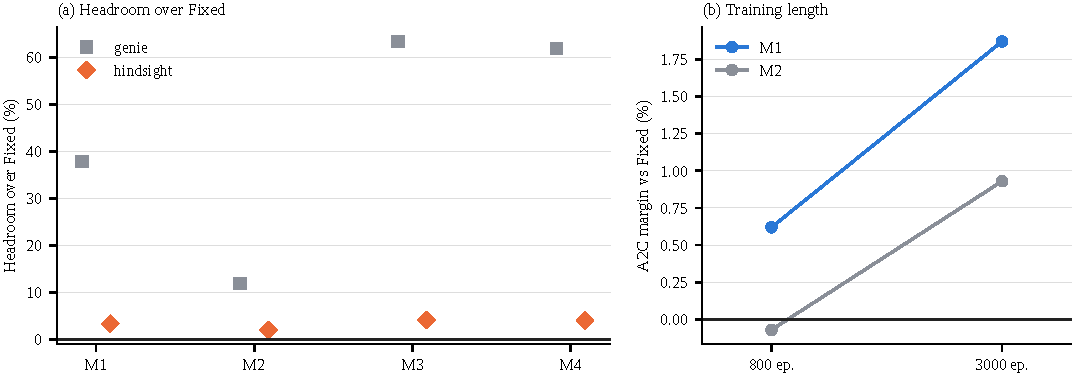
\includegraphics[width=\textwidth]{f5_headroom}
\caption{(a) Headroom over Fixed in the four cases: genie and per-trace hindsight bounds. (b) Margin of residual A2C over Fixed after \NCfgEpShort{} and \NCfgEpDl{} training episodes.}\label{fig:headroom}
\end{figure*}

\subsection{What the policy does}\label{sec:behaviour}
\subsubsection{Actions}
On \Gone{n_newtx_m1} scheduled new transmissions in M1 the policy raises the CQI by one step ($\delta=+\lit{1}$) in \NGoneAllPlus\,\% of decisions, keeps the base rule in \NGoneAllZero\,\% and lowers it in \NGoneAllMinus\,\% (Fig.~\ref{fig:policy}b). The ten policies differ widely: the share of upward steps ranges from \NGoneAllSeedMin{} to \NGoneAllSeedMax\,\% across seeds, although their on-time ratios are close. Three patterns hold in every seed. Upward steps are more frequent with one or two busy HARQ processes than with none (\NGoneBusyOnePlus\,\% against \NGoneBusyZeroPlus\,\%), when at most \NGoneSlackEdge{} of the deadline budget remains (\NGoneKSlackA\,\% against \NGoneSlackLoosePlus\,\%), and during interference bursts (\NGoneBurstPlus\,\% against \NGoneCalmPlus\,\%). This is consistent with a policy that accepts a higher block-error risk for a larger transport block when retransmissions are pending or the deadline is close. We have not tested this mechanism.

\subsubsection{Users at different speeds}
Splitting M1 by each user's mean speed and comparing with the original Context table shows an uneven gain (Fig.~\ref{fig:policy}a). Users between \NAoneEdgeLo{} and \NAoneEdgeHi~m/s gain \NAoneMidMar\,\% (hierarchical \NLevHier\,\% CI [\NAoneMidLo, \NAoneMidHi]\,\%) and faster users \NAoneFastMar\,\%. For users slower than \NAoneEdgeLo~m/s, \NAoneSlowShare\,\% of user-traces, the margin is \emph{negative}: \NAoneSlowMar\,\% ([\NAoneSlowLo, \NAoneSlowHi]\,\%). The policy's actions hardly depend on speed (\NGoneSpeedSlowPlus, \NGoneSpeedMidPlus{} and \NGoneSpeedFastPlus\,\% upward steps from the slowest to the fastest class). This is consistent with a largely speed-independent correction that helps when the channel ages quickly between report and use and over-shoots when it ages slowly. This breakdown was not repeated against the re-calibrated rules.

\begin{figure*}[t]
\centering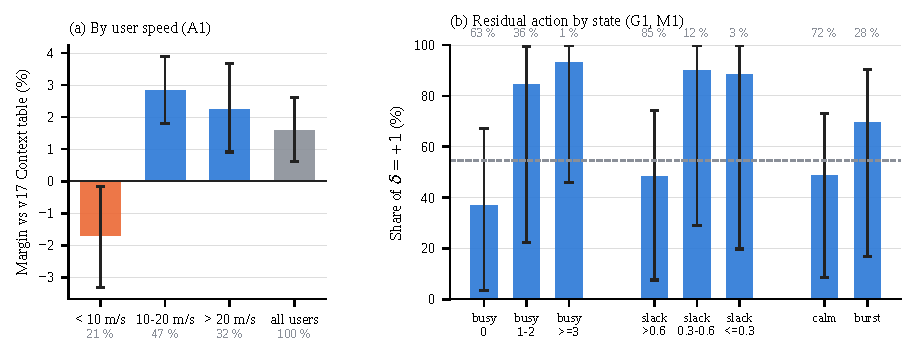
\includegraphics[width=\textwidth]{f7_policy}
\caption{What the policy does in M1. (a) Margin over the original Context table by user mean speed, with hierarchical \NLevHier\,\% CIs; gray labels give the share of user-traces. The all-user value pools user-traces, so it differs slightly from Table~\ref{tab:m1}. (b) Share of upward steps ($\delta=+\lit{1}$) on scheduled new transmissions by state, pooled over seeds (bars), with the minimum and maximum over the ten seeds (whiskers); gray labels give the share of decisions in each bin; dashed line: all decisions. Slack is the remaining fraction of the deadline budget.}\label{fig:policy}
\end{figure*}

\subsection{How much can learning add over a table?}\label{sec:hr1}
The results leave two questions open: why the goodput policy collapses to its base rule, and why a non-oracle base rule helps. A pre-registered analysis (HR1, Appendix~\ref{app:programme}) asks how much a learner could add, in one step, over the calibrated tables. It uses only logged decisions on the evaluation traces and adds no case to the multiplicity count.

\emph{Method.} For every scheduled new transmission we compute, through the simulator's link abstraction, the expected useful bits $q(a)$ of the first transmission (success probability times useful bits) for every offset $a$ that the tables can choose. A \emph{table} picks, in each of its cells, the offset with the best mean $q$. A \emph{learner} picks the offset with the best predicted $q$, where the prediction comes from gradient-boosted trees on the gNB-observable features that the policy sees. Both are cross-fitted (\NHRFolds{} folds, split by trace), so no decision is scored by a rule fitted on it. Two tree models were fixed in advance (gbt\_a and gbt\_b), and the larger estimate is reported; this was gbt\_a in every comparison. The \emph{residual} set restricts the learner to the base offset $\pm\lit{1}$, which is what the residual policy can do. Headroom is the relative gain of the learner (or of a genie that knows the true SINR) over the table, with \NLevHier\,\% intervals from \NHRBoot{} trace-level bootstrap replicates over \NHRDecisions{} decisions. \wordingsel{HR1scope}{HR1}{scope}{unrun}

\emph{How large is the room?} In M1, a genie that knows the true SINR would gain about \NHRGenieMoneHi\,\% over each calibrated table. This genie is per decision and in expected useful bits; it is not the trace-level genie bound of Fig.~\ref{fig:headroom}a. A learner that sees only the gNB-observable features could gain \NHRTabFullLo--\NHRTabFullHi\,\% with free choice of offset, and \NHRTabResLo--\NHRTabResHi\,\% when restricted to the base offset $\pm\lit{1}$. Around the decisions of the M1 policy, the residual headroom over the combined table is \NHRMoneComb\,\% ([\NHRMoneCombLo, \NHRMoneCombHi]\,\%). Fig.~\ref{fig:hr1} sets these values beside the observed margins. The two are not in the same units: headroom is myopic and counts expected useful bits of one first transmission, while a margin counts on-time packets or goodput over a whole trace, including retransmissions and queueing. We therefore compare them only qualitatively: in M1 the observed margins are well below the one-step headroom, and the combined table, which leaves the smallest observed margin, leaves only slightly less one-step headroom than the single-cue rules.

\begin{figure*}[t]
\centering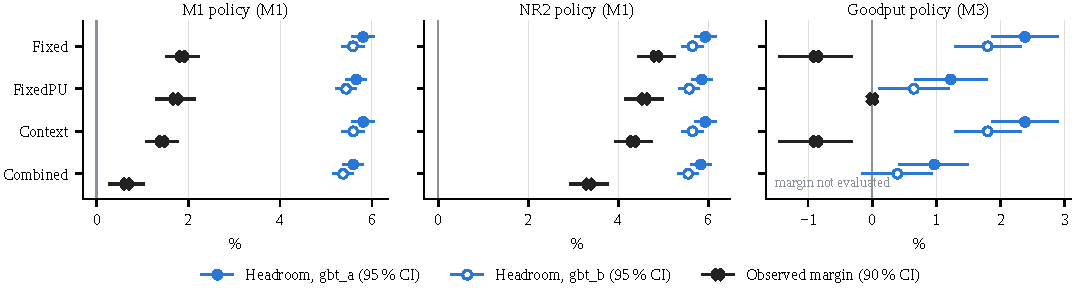
\includegraphics[width=\textwidth]{f12_hr1_headroom}
\caption{Learnable one-step headroom (residual set, base offset $\pm\lit{1}$) over each calibrated table, around the decisions of each learned policy, for both pre-specified estimators (\NLevHier\,\% bootstrap CI), beside the observed trace-level margin of that policy over the same comparator (\NLevTrace\,\% CI). M1 and NR2: comparators re-calibrated on \NGsixCalTraces{} traces; M3: original comparators, no combined table. Headroom is in expected useful bits of the first transmission and the margin in on-time ratio (M1) or goodput (M3), so the two are compared only qualitatively.}\label{fig:hr1}
\end{figure*}

\emph{Full-buffer goodput.} \wordingsel{HR1P1}{HR1}{verdict_P1}{unrun} The room is smaller than in M1 but not zero, and it remains against the base rule itself (FixedPU: \NHRMthreeFPU\,\%, [\NHRMthreeFPULo, \NHRMthreeFPUHi]\,\%). This leaves two explanations, and HR1 cannot separate them. Either the learner failed to find room that a one-step predictor finds, or the one-step gain is cancelled by costs that appear later, through HARQ retransmissions, queues or scheduling, which HR1 does not measure. We claim neither.

\emph{The non-oracle base.} \wordingsel{HR1P2}{HR1}{verdict_P2}{unrun} \wordingsel{HR1P3}{HR1}{verdict_P3}{unrun} The difference is small, however: \NHRPthreeEst{} points of headroom, against a realised difference of \NHRRealDiff{} points between the NR2 and M1 margins over the combined table (+\NRtwo{margin_ctxj} against \NGsixCtxJMar\,\%). The non-oracle base thus creates little extra one-step room. This is consistent with it mainly making the existing room easier to capture; HR1 does not test how.

\emph{Slow users.} \wordingsel{HR1P4}{HR1}{verdict_P4}{unrun} This prediction concerns the Context table on its own decisions, not the learned policy, and was not computed for the non-oracle configuration.

\emph{Second estimator.} With gbt\_b alone the four verdicts are the same: \NHRbPoneEst\,\% ([\NHRbPoneLo, \NHRbPoneHi]\,\%) for P1, \NHRbPtwoEst\,\% ([\NHRbPtwoLo, \NHRbPtwoHi]\,\%) for P2, \NHRbPthreeEst{} points ([\NHRbPthreeLo, \NHRbPthreeHi]) for P3 and \NHRbPfourEst{} points ([\NHRbPfourLo, \NHRbPfourHi]) for P4. Its estimates are lower throughout, so the size of the headroom depends on the predictor; the verdicts do not. The four intervals are not adjusted for multiplicity, and none of them changes a pre-registered claim of the paper.
